% ============================================================
%  PROPOSAL SKRIPSI — UNIVERSITAS KRISTEN KRIDA WACANA (UKRIDA)
%  Fakultas Ekonomi dan Bisnis — Program Studi S1 Manajemen
%  Konsentrasi: Manajemen Keuangan
%  Judul: Pengaruh Hedonic Motivation, Desire for Completeness, dan
%         Speculative Motive terhadap Impulsive Buying Booster Pack
%         Kartu Pokemon TCG dengan Self-Control sebagai Variabel Moderasi
%  Format: Sesuai Buku Pedoman Penyusunan Tugas Akhir FEB UKRIDA 2023 (Model B)
%  Engine: XeLaTeX (Font: Times New Roman via fontspec)
% ============================================================

\documentclass[12pt,a4paper]{article}

% ---- ENCODING & FONT (Pedoman UKRIDA §3.2.b: Times New Roman 12pt) ----
\usepackage{fontspec}
\setmainfont{Times New Roman}

% ---- CAPTION & ISTILAH INDONESIA ----
\renewcommand{\tablename}{Tabel}
\renewcommand{\figurename}{Gambar}

% ---- HYPHENATION & EMERGENCE STRETCH ----
\hyphenation{he-te-ro-ske-das-ti-si-tas mul-ti-ko-li-ne-a-ri-tas au-to-ko-re-la-si li-te-ra-si pe-ran-cang-an gra-ti-fi-ca-tion kom-ple-ti-tas}
\setlength{\emergencystretch}{2.5em}

% ---- PAGE GEOMETRY (Pedoman UKRIDA §3.2.a: Kiri 4cm, Atas/Kanan/Bawah 3cm) ----
\usepackage[
  left=4cm,
  right=3cm,
  top=3cm,
  bottom=3cm,
  a4paper
]{geometry}

% ---- LINE SPACING (Pedoman UKRIDA §3.2.e: 1.5 Spasi) ----
\usepackage{setspace}
\onehalfspacing

% ---- PARAGRAPH INDENT (Pedoman UKRIDA §3.2.f: 5 ketukan ~ 1.25cm) ----
\usepackage{indentfirst}
\setlength{\parindent}{1.25cm}
\setlength{\parskip}{0pt}
\usepackage{enumitem}

% ---- TABEL & ARRAY (Desain Terbuka Standar Jurnal / Booktabs) ----
\usepackage{booktabs}
\usepackage{longtable}
\usepackage{tabularx}
\usepackage{array}
\usepackage{multirow}
\usepackage{makecell}
\renewcommand{\arraystretch}{1.35}

% ---- GAMBAR & CAPTION (Pedoman UKRIDA §3.2.g: Tabel judul di atas, Gambar di bawah) ----
\usepackage{graphicx}
\usepackage{float}
\usepackage{caption}
\captionsetup[table]{labelsep=period, justification=raggedright, singlelinecheck=false, position=top, font=small}
\captionsetup[figure]{labelsep=period, justification=centering, position=bottom, font=small}

% ---- MATEMATIKA ----
\usepackage{amsmath}
\usepackage{amssymb}

% ---- TIKZ (DIAGRAM KERANGKA KONSEPTUAL) ----
\usepackage{tikz}
\usetikzlibrary{shapes.geometric, arrows.meta, positioning, calc}

% ---- SECTION TITLE FORMATTING (Pedoman UKRIDA §3.2.c: BAB KAPITAL BOLD CENTER) ----
\usepackage{titlesec}
\titleformat{\section}[block]
  {\normalfont\fontsize{12}{14}\bfseries\centering\MakeUppercase}
  {}
  {0pt}
  {}
\titlespacing*{\section}{0pt}{18pt}{12pt}

\titleformat{\subsection}[block]
  {\normalfont\fontsize{12}{14}\bfseries}
  {\thesubsection.}
  {0.5em}
  {}
\titlespacing*{\subsection}{0pt}{12pt}{6pt}

\titleformat{\subsubsection}[block]
  {\normalfont\fontsize{12}{14}\bfseries}
  {\thesubsubsection.}
  {0.5em}
  {}
\titlespacing*{\subsubsection}{0pt}{10pt}{4pt}

% ---- HEADER & FOOTER (Pedoman UKRIDA §3.3.b & Jeddy: Accent Bar 4 di Kanan Bawah) ----
\usepackage{fancyhdr}
\pagestyle{fancy}
\fancyhf{}
\renewcommand{\headrulewidth}{0pt}
\renewcommand{\footrulewidth}{0pt}
\fancyfoot[R]{\footnotesize\textbf{Universitas Kristen Krida Wacana} $|$ \thepage}

% Halaman awal frontmatter: footer kanan bawah dengan penomoran romawi kecil
\fancypagestyle{frontmatter}{
  \fancyhf{}
  \renewcommand{\headrulewidth}{0pt}
  \renewcommand{\footrulewidth}{0pt}
  \fancyfoot[R]{\footnotesize\textbf{Universitas Kristen Krida Wacana} $|$ \thepage}
}

% Halaman plain / bab baru: footer kanan bawah konsisten
\fancypagestyle{plain}{
  \fancyhf{}
  \renewcommand{\headrulewidth}{0pt}
  \renewcommand{\footrulewidth}{0pt}
  \fancyfoot[R]{\footnotesize\textbf{Universitas Kristen Krida Wacana} $|$ \thepage}
}

% ---- DAFTAR ISI / TABEL / GAMBAR (tocloft) ----
\usepackage[titles]{tocloft}
\renewcommand{\cfttoctitlefont}{\hfill\large\bfseries}
\renewcommand{\cftaftertoctitle}{\hfill}
\renewcommand{\cftlottitlefont}{\hfill\large\bfseries}
\renewcommand{\cftafterlottitle}{\hfill}
\renewcommand{\cftloftitlefont}{\hfill\large\bfseries}
\renewcommand{\cftafterloftitle}{\hfill}

% Awalan Tabel dan Gambar di daftar
\renewcommand{\cfttabpresnum}{Tabel }
\renewcommand{\cfttabaftersnum}{.}
\setlength{\cfttabnumwidth}{2.3cm}
\renewcommand{\cftfigpresnum}{Gambar }
\renewcommand{\cftfigaftersnum}{.}
\setlength{\cftfignumwidth}{2.5cm}

% ---- BIBLIOGRAPHY (APA Style via natbib + apalike) ----
\usepackage{natbib}
\bibliographystyle{apalike}
\bibpunct{(}{)}{;}{a}{,}{,}

% ---- HYPERREF (Tautan Interaktif Digital, Teks Hitam Formal Sesuai Pedoman §3.2.i) ----
\usepackage[
  colorlinks=true,
  linkcolor=black,
  citecolor=black,
  urlcolor=black,
  bookmarks=true,
  bookmarksnumbered=true,
  pdfpagemode=UseOutlines
]{hyperref}

% ---- PENOMORAN OTOMATIS BERDASARKAN BAB ----
\numberwithin{equation}{section}
\numberwithin{table}{section}
\numberwithin{figure}{section}

% ---- METADATA MAHASISWA & PEMBIMBING ----
\newcommand{\ukrida}{Universitas Kristen Krida Wacana}
\newcommand{\feb}{Fakultas Ekonomi dan Bisnis}
\newcommand{\prodi}{Program Studi S1 Manajemen}
\newcommand{\konsentrasi}{Manajemen Keuangan}
\newcommand{\namamahasiswa}{Arthur Reezan}
\newcommand{\nim}{312023002}
\newcommand{\dosbim}{Dr. Fredella Colline, S.E., M.M., CFP\textsuperscript{\textregistered}, PFM, CHCP-A}
\newcommand{\nidn}{[NIDN\_DOSEN]}
\newcommand{\ketprodi}{Rita Amelinda, S.E., M.M.}
\newcommand{\judulskripsi}{PENGARUH \emph{HEDONIC MOTIVATION}, \emph{DESIRE FOR COMPLETENESS}, DAN \emph{SPECULATIVE MOTIVE} TERHADAP \emph{IMPULSIVE BUYING} BOOSTER PACK KARTU POK\'EMON TCG DENGAN \emph{SELF-CONTROL} SEBAGAI VARIABEL MODERASI}

% ============================================================
%  DOKUMEN UTAMA
% ============================================================
\begin{document}

% ============================================================
%  BAGIAN AWAL — Penomoran Romawi Kecil
% ============================================================
\pagenumbering{roman}
\pagestyle{frontmatter}

% ------------------------------------------------------------
%  1. HALAMAN JUDUL LUAR / SAMPUL (hal. i)
% ------------------------------------------------------------
\thispagestyle{empty}
\begin{titlepage}
  \begin{center}
    \vspace*{0.5cm}
    {\large\bfseries PROPOSAL SKRIPSI}\\[1.2cm]

    {\large\bfseries
      PENGARUH \emph{HEDONIC MOTIVATION},\\
      \emph{DESIRE FOR COMPLETENESS}, DAN\\
      \emph{SPECULATIVE MOTIVE}\\
      TERHADAP \emph{IMPULSIVE BUYING} BOOSTER PACK\\
      KARTU POK\'EMON TCG DENGAN \emph{SELF-CONTROL}\\
      SEBAGAI VARIABEL MODERASI
    }\\[1.2cm]

    {\normalsize Diajukan Kepada \prodi}\\[0.2cm]
    {\normalsize Untuk Menyusun Skripsi Sarjana Manajemen (S.M.)}\\[1.2cm]

    {\normalsize Diajukan Oleh:}\\[0.4cm]
    {\large\bfseries \namamahasiswa}\\[0.2cm]
    {\large\bfseries (\nim)}\\[1.8cm]

    \vfill

    {\large\bfseries \feb}\\[0.3cm]
    {\large\bfseries \ukrida}\\[0.3cm]
    {\large\bfseries JAKARTA 2026}
  \end{center}
\end{titlepage}

\addtocounter{page}{1}

% ------------------------------------------------------------
%  2. HALAMAN PERNYATAAN KEASLIAN (hal. ii)
% ------------------------------------------------------------
\newpage
\thispagestyle{frontmatter}
\begin{center}
  {\large\bfseries PERNYATAAN KEASLIAN KARYA TUGAS AKHIR}
\end{center}

\vspace{0.3cm}
\noindent Saya mahasiswa \ukrida:

\vspace{0.15cm}
\noindent
\begin{tabular}{@{}lll@{}}
  Nama Mahasiswa & : & \namamahasiswa \\
  NIM            & : & \nim \\
  Program Studi  & : & \prodi \\
  Konsentrasi    & : & \konsentrasi \\
\end{tabular}

\vspace{0.3cm}
\noindent
Dengan ini menyatakan dengan sesungguhnya bahwa Proposal Skripsi yang berjudul:

\vspace{0.15cm}
\begin{center}
  \bfseries``\judulskripsi''
\end{center}

\vspace{0.15cm}
\noindent adalah:

\begin{enumerate}[topsep=2pt,itemsep=2pt,partopsep=0pt,parsep=0pt]
  \item Benar-benar hasil karya saya sendiri, bukan merupakan jiplakan, plagiarisme, fabrikasi, atau tiruan dari karya tulis ilmiah orang lain yang pernah diajukan untuk memperoleh gelar akademik di perguruan tinggi manapun.
  \item Seluruh kutipan, data, dan rujukan ilmiah yang digunakan dalam naskah ini telah dicantumkan sumbernya secara jelas dan lengkap sesuai dengan kaidah penulisan ilmiah yang berlaku di \ukrida.
  \item Apabila di kemudian hari terbukti bahwa pernyataan ini tidak benar atau ditemukan indikasi plagiarisme, saya bersedia menerima sanksi akademik yang berlaku sesuai dengan peraturan perundang-undangan dan ketentuan di lingkungan Universitas Kristen Krida Wacana.
\end{enumerate}

\vspace{0.5cm}
\noindent
\hfill
\begin{minipage}[t]{6.5cm}
  \centering
  Jakarta, \underline{\hspace{3.5cm}} 2026\\[0.25cm]
  Yang menyatakan,\\[0.35cm]
  \framebox(70,45){\begin{minipage}{2.2cm}\centering\scriptsize\itshape Meterai\\Rp10.000\end{minipage}}\\[0.45cm]
  \textbf{(\namamahasiswa)}\\
  NIM: \nim
\end{minipage}

% ------------------------------------------------------------
%  3. HALAMAN PERSETUJUAN PROPOSAL SKRIPSI (hal. iii)
%  (Format Sesuai Lampiran 2 Buku Pedoman Penyusunan Tugas Akhir FEB UKRIDA 2023)
% ------------------------------------------------------------
\newpage
\thispagestyle{frontmatter}
\begin{center}
  {\large\bfseries PERSETUJUAN PROPOSAL SKRIPSI}
\end{center}

\vspace{0.6cm}
\noindent
\begin{tabular}{lll}
  Nama          & : & \namamahasiswa \\
  N.I.M.        & : & \nim \\
  Program Studi & : & \prodi \\
  Konsentrasi   & : & \konsentrasi \\
\end{tabular}

\vspace{0.5cm}
\noindent \textbf{Judul yang Diajukan:}

\vspace{0.2cm}
\begin{flushleft}
  \bfseries\judulskripsi
\end{flushleft}

\vspace{0.8cm}
\noindent Jakarta, \underline{\hspace{3cm}} 2026

\vspace{0.6cm}
\noindent Menyetujui,

\vspace{0.4cm}
\noindent
\begin{tabular}{p{6.5cm} p{6.5cm}}
  Dosen Pembimbing & Dosen Pendamping \\[2.2cm]
  \textbf{(\dosbim)} & (\underline{\hspace{4cm}}) \\
  NIDN: \nidn & \\
\end{tabular}

\vspace{0.8cm}
\noindent Mengetahui,

\vspace{0.4cm}
\noindent
\begin{tabular}{l}
  \textbf{(\ketprodi)} \\
  Ketua Program Studi S1 Manajemen
\end{tabular}

% ------------------------------------------------------------
%  4. HALAMAN PENGESAHAN TIM PENGUJI (hal. iv)
% ------------------------------------------------------------
\newpage
\thispagestyle{frontmatter}
\begin{center}
  {\large\bfseries PENGESAHAN TIM PENGUJI SEMINAR PROPOSAL SKRIPSI}\\[0.5cm]
  {\normalsize Proposal Skripsi dengan Judul:}\\[0.3cm]
  {\bfseries\judulskripsi}\\[0.5cm]
  {\normalsize Diajukan Oleh:}\\[0.2cm]
  {\large\bfseries \namamahasiswa}\\[0.1cm]
  {\large\bfseries (\nim)}
\end{center}

\vspace{0.4cm}
\noindent
Telah dipertahankan di hadapan Tim Penguji Seminar Proposal Skripsi Program Studi S1 Manajemen Fakultas Ekonomi dan Bisnis Universitas Kristen Krida Wacana pada:

\vspace{0.4cm}
\noindent \textbf{Hari / Tanggal Seminar:} \underline{\hspace{4cm}}, \underline{\hspace{3cm}} 2026

\vspace{0.4cm}
\noindent \textbf{Tim Penguji Seminar Proposal:}

\vspace{0.4cm}
\noindent
\begin{tabular}{@{}p{0.5cm} >{\raggedright\arraybackslash}p{3.2cm} p{0.2cm} >{\raggedright\arraybackslash}p{5.0cm} p{2.8cm}@{}}
  1. & Ketua Penguji    & : & \underline{\hspace{4.4cm}} & ( \underline{\hspace{2.3cm}} ) \\[1.3cm]
  2. & Anggota Penguji  & : & \underline{\hspace{4.4cm}} & ( \underline{\hspace{2.3cm}} ) \\[1.3cm]
  3. & Dosen Pembimbing & : & \dosbim                    & ( \underline{\hspace{2.3cm}} ) \\
\end{tabular}

% ------------------------------------------------------------
%  5. KATA PENGANTAR (hal. v)
% ------------------------------------------------------------
\newpage
\thispagestyle{frontmatter}
\begin{center}
  {\large\bfseries KATA PENGANTAR}
\end{center}

\vspace{0.4cm}
Puji dan syukur penulis panjatkan ke hadirat Tuhan Yang Maha Esa atas kasih, anugerah, dan penyertaan-Nya yang senantiasa melimpah, sehingga penulis dapat menyelesaikan penyusunan proposal skripsi yang berjudul \textbf{``\judulskripsi''} dengan baik, lancar, dan tepat waktu.

Proposal skripsi ini disusun sebagai salah satu tahapan akademik yang diwajibkan dalam rangka menempuh ujian seminar proposal guna menyelesaikan studi pada Program Studi S1 Manajemen, Konsentrasi Manajemen Keuangan, Fakultas Ekonomi dan Bisnis, Universitas Kristen Krida Wacana (UKRIDA), Jakarta.

Dalam proses penyusunan naskah proposal ini, penulis mendapatkan banyak bimbingan, arahan metodologis, dukungan moril, serta fasilitas dari berbagai pihak. Oleh karena itu, dengan penuh rasa hormat dan kerendahan hati, penulis menyampaikan terima kasih dan apresiasi yang setinggi-tingginya kepada:

\begin{enumerate}
  \item \textbf{\dosbim}, selaku Dosen Pembimbing Skripsi, yang telah dengan luar biasa sabar, teliti, kritis, dan penuh dedikasi meluangkan waktu serta mencurahkan tenaga dan pikiran dalam membimbing, mengarahkan, dan menyempurnakan naskah proposal ini sejak tahap awal perumusan gagasan hingga penyusunan naskah komprehensif.
  \item \textbf{\ketprodi}, selaku Ketua Program Studi S1 Manajemen FEB UKRIDA, atas segala arahan, kemudahan proses administratif, dan bimbingan akademik yang diberikan.
  \item \textbf{Bapak dan Ibu Dosen Penguji Seminar Proposal}, yang telah bersedia meluangkan waktu untuk menguji, memberikan koreksi kritis, serta masukan yang konstruktif guna menyempurnakan naskah penelitian ini.
  \item \textbf{Seluruh Dosen dan Staf Pengajar FEB UKRIDA}, yang telah membagikan ilmu pengetahuan, wawasan analisis keuangan, serta etika profesional selama masa perkuliahan penulis.
  \item \textbf{Kedua Orang Tua dan Keluarga Tercinta}, atas doa yang tiada putus, limpahan kasih sayang, ketulusan pengorbanan, serta dorongan moral dan material yang menjadi sumber kekuatan utama bagi penulis.
  \item \textbf{Rekan-rekan Mahasiswa Manajemen FEB UKRIDA Angkatan 2023} dan sahabat seperjuangan, atas diskusi yang membangun, motivasi, dan kerja sama selama proses perkuliahan.
  \item \textbf{Komunitas Kolektor dan Pemain Pok\'emon TCG di Indonesia}, yang telah memberikan gambaran nyata mengenai fenomena pasar kartu koleksi di lapangan.
\end{enumerate}

Penulis menyadari bahwa proposal ini masih jauh dari kesempurnaan. Kritik dan saran yang membangun sangat diharapkan demi penyempurnaan karya ilmiah ini ke depan. Semoga proposal skripsi ini dapat memberikan manfaat akademis dan praktis bagi perkembangan kajian ilmu manajemen keuangan perilaku di Indonesia.

\vspace{0.6cm}
\noindent
\hfill
\begin{minipage}[t]{5.5cm}
  Jakarta, \underline{\hspace{3.2cm}} 2026\\[0.25cm]
  \textbf{Penulis},\\[1.8cm]
  \textbf{\namamahasiswa}\\
  NIM: \nim
\end{minipage}

% ------------------------------------------------------------
%  6. ABSTRAK (hal. vi)
% ------------------------------------------------------------
\newpage
\thispagestyle{frontmatter}
\begin{singlespace}
\begin{center}
  {\large\bfseries ABSTRAK}\\[0.3cm]
  {\bfseries\judulskripsi}\\[0.3cm]
  {\bfseries\namamahasiswa\ (\nim)}\\[0.1cm]
  {\footnotesize \prodi, \feb, \ukrida}\\[0.1cm]
  {\footnotesize Dosen Pembimbing: \dosbim}
\end{center}

\vspace{0.25cm}
Penelitian ini bertujuan untuk menganalisis dan menguji secara empiris pengaruh \emph{hedonic motivation} (motivasi hedonis), \emph{desire for completeness} (hasrat kelengkapan koleksi), dan \emph{speculative motive} (motif spekulasi finansial) terhadap \emph{impulsive buying} (pembelian impulsif) \emph{booster pack} kartu Pok\'emon Trading Card Game (Pok\'emon TCG) fisik resmi berbahasa Indonesia, serta menguji peran kontrol diri (\emph{self-control}) sebagai variabel moderasi dalam memperlemah pengaruh ketiga variabel anteseden tersebut.

Penelitian ini menggunakan pendekatan kuantitatif asosiatif dengan desain survei \emph{cross-sectional}. Data primer dikumpulkan melalui penyebaran kuesioner daring berbasis skala Likert 5 poin kepada responden yang dipilih melalui teknik \emph{purposive sampling}. Kriteria inklusi sampel adalah konsumen atau kolektor Warga Negara Indonesia (WNI) berusia minimal 17 tahun yang pernah membeli \emph{booster pack} Pok\'emon TCG fisik resmi dalam rentang waktu 6--12 bulan terakhir. Jumlah sampel yang ditargetkan adalah 120 hingga 150 responden, mengacu pada rekomendasi ukuran sampel \citet{green1991subjects} dan \citet{cohen1988statistical} untuk mencapai kekuatan uji statistik (\emph{statistical power}) yang memadai pada model regresi linear berganda. Metode analisis data menggunakan analisis regresi berganda dan \emph{Moderated Regression Analysis} (MRA) dengan prosedur standarisasi skor rata-rata (\emph{mean-centering}) guna mengatasi potensi multikolinearitas struktural antar-istilah interaksi \citep{aiken1991multiple, ghozali2018aplikasi}, yang diolah menggunakan perangkat lunak IBM SPSS Statistics.

Penelitian ini menawarkan kebaruan teoritis (\emph{novelty}) dengan mengintegrasikan kerangka psikologi lingkungan \emph{Stimulus-Organism-Response} (S-O-R), psikologi kolektor (\emph{Zeigarnik Effect} dan \emph{The Completing the Set Effect}), teori regulasi diri (\emph{Self-Regulation Theory}), serta prinsip-prinsip keuangan perilaku (\emph{behavioral finance}) pada fenomena komoditas hobi fisik bernilai spekulatif tinggi. Hasil penelitian ini diharapkan memberikan kontribusi empiris bagi konsumen muda dalam menjaga kontrol diri finansial, serta masukan aplikatif bagi komunitas hobi dan pemangku kebijakan edukasi keuangan generasi muda di Indonesia.

\vspace{0.3cm}
\noindent\textbf{Kata Kunci:} \emph{Impulsive Buying}, \emph{Hedonic Motivation}, \emph{Desire for Completeness}, \emph{Speculative Motive}, \emph{Self-Control}, \emph{Moderated Regression Analysis}, Pok\'emon TCG, Keuangan Perilaku (\emph{Behavioral Finance}).
\end{singlespace}

% ------------------------------------------------------------
%  7. ABSTRACT (hal. vii)
%  (Format Sesuai Lampiran 9 Buku Pedoman FEB UKRIDA)
% ------------------------------------------------------------
\newpage
\thispagestyle{frontmatter}
\begin{singlespace}
\begin{center}
  {\large\bfseries ABSTRACT}\\[0.2cm]
  {\bfseries THE EFFECT OF HEDONIC MOTIVATION, DESIRE FOR COMPLETENESS, AND SPECULATIVE MOTIVE ON IMPULSIVE BUYING OF POK\'EMON TCG BOOSTER PACKS WITH SELF-CONTROL AS A MODERATING VARIABLE}\\[0.2cm]
  {\bfseries\namamahasiswa\ (\nim)}\\[0.05cm]
  {\footnotesize Undergraduate Program in Management, Faculty of Economics and Business, UKRIDA}\\[0.05cm]
  {\footnotesize Thesis Advisor: \dosbim}
\end{center}

\vspace{0.15cm}
\emph{This research aims to analyze and empirically test the effects of hedonic motivation, desire for completeness, and speculative motive on the impulsive buying behavior of official Indonesian-language physical Pok\'emon Trading Card Game (Pok\'emon TCG) booster packs, as well as to evaluate the moderating role of self-control in weakening the relationships between these three antecedent variables and impulsive buying.}

\emph{This study adopts an associative quantitative approach utilizing a cross-sectional survey design. Primary data are gathered via self-administered online questionnaires employing a 5-point Likert scale, distributed to respondents selected through purposive sampling. The sample inclusion criteria comprise Indonesian citizens aged 17 and above who have purchased official physical booster packs within the past 6 to 12 months. The targeted sample size ranges from 120 to 150 respondents, consistent with the statistical power criteria established by \citet{green1991subjects} and \citet{cohen1988statistical} for multiple regression frameworks. The empirical model is estimated using multiple linear regression and Moderated Regression Analysis (MRA) with mean-centering procedures to eliminate structural multicollinearity \citep{aiken1991multiple, ghozali2018aplikasi}, executed via IBM SPSS Statistics software.}

\emph{This study provides theoretical novelty by synthesizing the Stimulus-Organism-Response (S-O-R) paradigm, collector psychology (the Zeigarnik Effect and The Completing the Set Effect), Self-Regulation Theory, and behavioral finance principles in the context of tangible alternative assets exhibiting volatile secondary market premiums. The findings are expected to offer practical insights for young consumers in exercising financial discipline regarding discretionary collectibles and provide strategic inputs for community organizers and financial educators targeting Generation Z.}

\vspace{0.2cm}
\noindent\textbf{\emph{Keywords:}} \emph{Impulsive Buying, Hedonic Motivation, Desire for Completeness, Speculative Motive, Self-Control, Moderated Regression Analysis, Pok\'emon TCG, Behavioral Finance.}

\vspace{0.35cm}
\noindent
\begin{tabular}{@{}p{6.6cm} p{6.6cm}@{}}
  Mahasiswa & Dosen Pembimbing \\[1.1cm]
  \textbf{(\namamahasiswa)} & \textbf{(\dosbim)} \\
  NIM: \nim & NIDN: \nidn
\end{tabular}
\end{singlespace}

% ------------------------------------------------------------
%  8. DAFTAR ISI (hal. viii)
% ------------------------------------------------------------
\newpage
\thispagestyle{frontmatter}
\renewcommand{\contentsname}{DAFTAR ISI}
\tableofcontents
\addtocontents{toc}{\protect\thispagestyle{frontmatter}}

% ------------------------------------------------------------
%  9. DAFTAR TABEL (hal. ix)
% ------------------------------------------------------------
\newpage
\thispagestyle{frontmatter}
\renewcommand{\listtablename}{DAFTAR TABEL}
\listoftables
\addcontentsline{toc}{section}{DAFTAR TABEL}
\addtocontents{lot}{\protect\thispagestyle{frontmatter}}

% ------------------------------------------------------------
%  10. DAFTAR GAMBAR (hal. x)
% ------------------------------------------------------------
\newpage
\thispagestyle{frontmatter}
\renewcommand{\listfigurename}{DAFTAR GAMBAR}
\listoffigures
\addcontentsline{toc}{section}{DAFTAR GAMBAR}
\addtocontents{lof}{\protect\thispagestyle{frontmatter}}

% ============================================================
%  BAGIAN INTI / UTAMA — Penomoran Angka Arab (Mulai hal. 1)
% ============================================================
\newpage
\pagenumbering{arabic}
\pagestyle{fancy}

% ============================================================
%  BAB 1: PENDAHULUAN
% ============================================================
\setcounter{section}{0}
\section*{BAB 1\\[0.3cm]PENDAHULUAN}
\addcontentsline{toc}{section}{\texorpdfstring{BAB 1\quad PENDAHULUAN}{BAB 1 PENDAHULUAN}}
\setcounter{section}{1}
\setcounter{subsection}{0}
\setcounter{table}{0}
\setcounter{figure}{0}
\setcounter{equation}{0}

\subsection{Latar Belakang Penelitian}

Waralaba media (\emph{media franchise}) Pok\'emon yang diciptakan oleh Satoshi Tajiri bersama Game Freak dan diluncurkan oleh Nintendo pada tahun 1996 di Jepang telah berkembang menjadi fenomena budaya pop global paling berpengaruh di dunia. Berdasarkan data agregasi industri media internasional, Pok\'emon dinobatkan sebagai waralaba media dengan pendapatan tertinggi sepanjang masa (\emph{the highest-grossing media franchise in history}), dengan estimasi pendapatan kotor kumulatif melampaui US\$ 100 miliar. Angka ini melampaui waralaba legendaris dunia lainnya seperti \emph{Star Wars}, \emph{Marvel Cinematic Universe}, maupun \emph{Mickey Mouse}. Keberhasilan masif ini dibangun di atas fondasi ekosistem multimedia yang saling memperkuat:
\begin{enumerate}
  \item \textbf{Lini Permainan Video (\emph{Video Games}):} Dimulai dari RPG Generasi I (\emph{Pok\'emon Red/Green/Blue}) di konsol Nintendo Game Boy hingga Generasi IX (\emph{Pok\'emon Scarlet/Violet}) di Nintendo Switch, serta revolusi permainan seluler berbasis \emph{Augmented Reality} \emph{Pok\'emon GO} yang memecahkan rekor interaksi ratusan juta pemain global secara simultan, disusul inovasi digital mutakhir seperti \emph{Pok\'emon Sleep}, \emph{Pok\'emon UNITE}, dan \emph{Pok\'emon Trading Card Game Pocket}.
  \item \textbf{Lini Animasi dan Film Bioskop:} Serial televisi anime yang mengisahkan 25 tahun perjalanan Satoshi (Ash Ketchum) dan Pikachu yang telah ditayangkan di lebih dari 190 negara, deretan film layar lebar monumental seperti \emph{Pok\'emon: The First Movie -- Mewtwo Strikes Back} (1998) yang merajai \emph{box office} dunia, film aksi langsung (\emph{live-action}) Hollywood berpendapatan tinggi \emph{Pok\'emon Detective Pikachu} (2019), hingga serial anime generasi terbaru \emph{Pok\'emon Horizons}.
  \item \textbf{Lini Lisensi, Merchandise, dan Gerai Ritel:} Jaringan gerai resmi \emph{Pok\'emon Center} di berbagai kota metropolitan dunia serta penyelenggaraan turnamen tahunan bergengsi berskala internasional yakni \emph{Pok\'emon World Championships}.
\end{enumerate}

Di antara seluruh pilar ekosistem multimedia tersebut, \textbf{permainan kartu fisik atau \emph{Pok\'emon Trading Card Game} (Pok\'emon TCG)} memegang peranan yang paling sentral, monumental, dan memiliki perputaran ekonomi koleksi fisik (\emph{physical collectibles}) terbesar di dunia. Hingga tahun 2024, The Pok\'emon Company mencatat bahwa produksi kumulatif kartu Pok\'emon fisik telah menembus lebih dari 52,9 miliar lembar kartu yang didistribusikan ke 93 wilayah dan diterjemahkan ke dalam 14 bahasa. Kartu Pok\'emon bukan lagi sekadar alat permainan meja (\emph{tabletop game}) anak-anak, melainkan telah bertransformasi menjadi \textbf{instrumen aset alternatif koleksi (\emph{alternative collectibles asset})} bernilai ekonomi tinggi yang diperdagangkan secara aktif oleh kalangan dewasa muda, investor hobi, dan balai lelang global.

Di Indonesia, kehadiran kartu resmi Pok\'emon TCG berbahasa Indonesia sejak tahun 2019 melalui The Pok\'emon Company bekerja sama dengan AKG Games (PT Adiperkasa Citra Lestari) mengalami akselerasi luar biasa. Strategi distribusinya sangat unik dan agresif: produk kartu tidak hanya dipasarkan melalui toko hobi khusus (\emph{Local Game Stores} / LGS), melainkan didistribusikan secara masif di ribuan gerai jaringan ritel modern minimarket terkemuka (Indomaret, Alfamart, Gramedia, Toys Kingdom). Penempatan produk kartu langsung di etalase meja kasir ritel modern ini berhasil mendemokratisasi akses dan mengubah hobi kartu dari komunitas ceruk (\emph{niche}) menjadi fenomena konsumsi populer berskala nasional. Minat masyarakat Indonesia—khususnya kalangan mahasiswa dan Generasi Z—terhadap kartu fisik ini didorong oleh konvergensi antara fungsi rekreasi permainan, prestise sosial, hobi mengoleksi kartu langka, serta motif spekulasi finansial.

Dinamika pasar Pok\'emon TCG fisik di Indonesia memunculkan fenomena perilaku konsumsi yang sangat unik sekaligus problematis. Produk kartu fisik dijual dalam format kemasan acak tertutup (\emph{blind pack} atau \emph{booster pack}) dengan harga eceran resmi yang sangat terjangkau, berkisar antara Rp20.000 hingga Rp30.000 per bungkus (berisi 5 lembar kartu acak). Namun, di dalam bungkus tersebut tersimpan peluang probabilitas untuk menarik kartu dengan tingkat kelangkaan tinggi (\emph{Special Illustration Rare / SAR}, kartu \emph{Super Rare / SR}, atau \emph{Ultra Rare / UR}). Di pasar sekunder daring (Tokopedia, Shopee, grup lelang Facebook, dan komunitas media sosial), kartu-kartu berkarakter favorit (seperti Charizard, Pikachu, atau kartu pelatih wanita/waifu populer) diperjualbelikan dengan harga fantastis mulai dari ratusan ribu hingga puluhan juta rupiah per lembar.

Fenomena disparitas harga pasar sekunder ini diperkuat oleh keberadaan industri \textbf{sertifikasi penilaian kondisi fisik kartu (\emph{card grading})}. Lembaga grading independen berstandar internasional terkemuka seperti \textbf{PSA (\emph{Professional Sports Authenticator})}, \textbf{BGS (\emph{Beckett Grading Services})}, dan \textbf{CGC Cards} memeriksa integritas fisik kartu secara mikroskopis berdasarkan empat kriteria utama: \emph{centering} (kesimetrisan cetak), \emph{surface} (kebersihan permukaan tanpa goresan), \emph{edges} (kerapian tepi), dan \emph{corners} (ketajaman sudut kartu). Kartu yang memenuhi kesempurnaan tertinggi akan disegel permanen dalam wadah akrilik kedap udara (\emph{tamper-evident slab}) dan diberi label skor kualitas 1 hingga 10 (\emph{PSA 10 Gem Mint} atau \emph{BGS 10 Pristine}). Kartu berpredikat \emph{Gem Mint 10} secara instan bertransformasi menjadi aset terstandardisasi yang likuid di bursa lelang global dengan harga jual yang melonjak 5 kali hingga 50 kali lipat dibandingkan kartu mentah (\emph{raw card}). Kehadiran pasar grading ini memicu gelombang spekulasi (\emph{grading arbitrage}), di mana konsumen tergiur membeli \emph{booster pack} murah dengan harapan menarik kartu berkondisi sempurna untuk digrade dan dijual kembali demi mendulang keuntungan modal (\emph{capital gain}).

Disparitas nilai yang ekstrem dan mekanisme kemasan acak berbasis probabilitas (\emph{gacha mechanism}) tersebut mendorong antusiasme transaksi yang berlebihan. Setiap kali ekspansi seri baru diluncurkan (seperti Seri 151, Kilau Hitam, atau Terastal), gerai ritel modern kerap diserbu antrean pembeli dan produk ludes terjual dalam hitungan jam. Banyak pembeli melakukan transaksi pembelian \emph{booster pack} secara berulang-ulang, mendadak di kasir toko, dan tidak direncanakan sebelumnya dalam alokasi anggaran bulanan. Transaksi belanja yang tiba-tiba, didorong oleh letupan emosional sesaat, dan mengabaikan pertimbangan rasional ini mengindikasikan terjadinya gejala \textbf{pembelian impulsif (\emph{impulsive buying})} yang masif pada komoditas kartu Pok\'emon fisik di Indonesia.

Fenomena \emph{impulsive buying} telah lama menjadi pusat perhatian utama dalam literatur perilaku konsumen dan psikologi ekonomi. \citet{stern1962significance} dalam karya klasiknya mengklasifikasikan pembelian impulsif ke dalam empat kategori: \emph{pure impulse}, \emph{reminder impulse}, \emph{suggestion impulse}, dan \emph{planned impulse buying}. \citet{rook1987buying} mendefinisikan \emph{impulsive buying} sebagai desakan pembelian yang terjadi seketika, kuat, dan persisten tanpa adanya pertimbangan kognitif sadar sebelumnya mengenai konsekuensi pengeluaran. Lebih lanjut, \citet{beatty1998impulse} serta studi meta-analisis komprehensif oleh \citet{amos2014meta} mengungkapkan bahwa keputusan pembelian impulsif sesungguhnya merupakan muara perilaku yang dipengaruhi oleh spektrum faktor penentu (\emph{antecedents}) yang sangat luas dalam literatur ilmiah terdahulu:
\begin{enumerate}
  \item \textbf{Faktor Emosional dan Afektif (\emph{Affective Drivers}):} Meliputi motivasi berbelanja untuk kesenangan (\emph{hedonic shopping motivations}), pencarian pelepasan stres dan petualangan (\citealp{babin1994work}; \citealp{arnold2003hedonic}), suasana hati positif (\emph{positive affect}), serta luapan kegembiraan sesaat (\emph{excitement and arousal}) (\citealp{gueltekin2012influence}).
  \item \textbf{Faktor Kognitif dan Psikologi Kolektor (\emph{Cognitive and Collector Drivers}):} Meliputi ketegangan mental ketidaktuntasan himpunan (\emph{Zeigarnik Effect}) \citep{zeigarnik1927behalten}, dorongan psikologis melengkapi set koleksi (\emph{The Completing the Set Effect}) \citep{gao2014completing}, pembingkaian himpunan semu (\emph{Pseudo-Set Framing}) \citep{barasz2017pseudo}, serta hasrat kepemilikan materialistik atas objek langka \citep{belk1995collecting}.
  \item \textbf{Faktor Finansial dan Spekulasi Pasar (\emph{Economic and Speculative Drivers}):} Meliputi ekspektasi apresiasi nilai modal (\emph{capital gain}), likuiditas pasar sekunder, anomali psikologi pasar modal dan bias optimisme berlebihan (\emph{overoptimism bias}) \citep{shiller2000irrational, baur2018bitcoin}, persepsi memenangkan lotre (\emph{gambler's fallacy}), serta bias perilaku investor muda \citep{colline2024biases}.
  \item \textbf{Faktor Situasional dan Rangsangan Toko (\emph{Situational and Atmospheric Drivers}):} Meliputi mekanisme kejutan kemasan tertutup (\emph{blind pack mystery}), display etalase kasir yang memancing sentuhan fisik (\emph{need for touch}) \citep{peck2006if}, diskon promosi sesaat, serta desakan kelangkaan stok fisik \citep{amos2014meta}.
\end{enumerate}

Berdasarkan pemetaan komprehensif faktor-faktor penentu \emph{impulsive buying} dalam literatur di atas, penelitian ini secara deduktif memilih dan memfokuskan pada tiga variabel independen utama yang paling tepat merepresentasikan karakteristik intrinsik dan perilaku konsumsi komoditas kartu Pok\'emon TCG:
\begin{enumerate}
  \item Pertama, \textbf{faktor afektif diwakili oleh \emph{Hedonic Motivation} ($X_1$)}. Konsumen membeli \emph{booster pack} bukan untuk pemenuhan kebutuhan utiliter harian, melainkan demi mengejar kepuasan emosional, sensasi hiburan, dan lonjakan dopamin saat merobek bungkus foil kemasan (\emph{pack opening thrill}) \citep{arnold2003hedonic, gueltekin2012influence}.
  \item Kedua, \textbf{faktor psikologis koleksi diwakili oleh \emph{Desire for Completeness} ($X_2$)}. Berakar pada \emph{Zeigarnik Effect} \citep{zeigarnik1927behalten, belk1995collecting} dan formalisasi \emph{The ``Completing the Set'' Effect} \citep{gao2014completing, barasz2017pseudo}, binder album kolektor yang masih memiliki slot nomor kosong menciptakan ketegangan kognitif internal. Hasrat menuntaskan set secara utuh memicu dorongan psikologis mendesak untuk terus membeli bungkus kartu tambahan secara spontan demi menutup celah kekosongan tersebut.
  \item Ketiga, \textbf{faktor ekonomi dan pasar diwakili oleh \emph{Speculative Motive} ($X_3$)}. Dalam perspektif \emph{behavioral finance}, transaksi kartu Pok\'emon fisik sangat diwarnai oleh motif spekulasi finansial \citep{shiller2000irrational, baur2018bitcoin, colline2024biases}. Pembeli tergiur oleh likuiditas pasar lelang daring dan tren grading PSA/BGS, memicu keyakinan bahwa modal kecil membeli beberapa \emph{pack} berpeluang menghasilkan kartu langka bernilai jutaan rupiah untuk dijual kembali (\emph{capital gain}).
\end{enumerate}

Terkait pengukuran variabel dependen \emph{Impulsive Buying} ($Y$), literatur perilaku konsumen mengenal beberapa instrumen pengukuran teruji, antara lain skala unidimensional pengaruh normatif oleh \citet{rook1995normative} serta skala dorongan belanja impulsif dalam toko oleh \citet{beatty1998impulse}. Namun, penelitian ini mengadopsi instrumen pengukuran multidimensional \citet{verplanken2001individual} yang disintesis dengan definisi operasional \citet{rook1987buying}. Skala ini membedakan secara tegas antara dimensi kognitif (ketiadaan perencanaan belanja dan pengabaian dampak keuangan) dan dimensi afektif (luapan kegembiraan mendadak dan dorongan spontan). Pemilihan instrumen ini didasarkan pada pertimbangan bahwa perilaku pembelian \emph{booster pack} kartu di etalase ritel melibatkan pergulatan nyata antara sensasi afektif merobek kemasan dengan kelalaian kognitif terhadap alokasi anggaran pribadi.

Meskipun ketiga faktor pendorong ($X_1, X_2, X_3$) secara teoretis berkaitan erat dengan keputusan belanja, telaah mendalam terhadap riset-riset empiris terdahulu justru memperlihatkan adanya kesenjangan penelitian (\emph{empirical research gap}) berupa temuan yang saling bertolak belakang (\emph{inconsistent findings}):
\begin{itemize}
  \item Pada pengaruh \emph{Hedonic Motivation} terhadap \emph{Impulsive Buying}, sejumlah peneliti membuktikan pengaruh positif signifikan karena dorongan kesenangan emosional langsung melumpuhkan kalkulasi rasional konsumen \citep{arnold2003hedonic, gueltekin2012influence, pranggabayu2022pengaruh}. Namun, penelitian lain menemukan hasil tidak signifikan ketika faktor kendala anggaran dan pertimbangan utilitas fungsional mendominasi keputusan konsumen \citep{zheng2019impact, prasetio2021hedonic}.
  \item Pada pengaruh \emph{Desire for Completeness} terhadap \emph{Impulsive Buying}, \citet{gao2014completing} dan \citet{barasz2017pseudo} menemukan bahwa hasrat melengkapi kesatuan himpunan memicu percepatan belanja yang agresif dan spontan. Sebaliknya, studi klasik perilaku kolektor oleh \citet{long2000consuming} dan \citet{spero2004approach} menemukan bahwa kolektor berpengalaman (\emph{mature collectors}) justru menumbuhkan kehati-hatian finansial; mereka menahan diri dari belanja spekulatif pada kemasan acak dan lebih memilih strategi pembelian terencana pada kartu satuan (\emph{single cards}) di pasar sekunder.
  \item Pada pengaruh \emph{Speculative Motive} terhadap \emph{Impulsive Buying}, \citet{shiller2000irrational} dan \citet{aryadi2024personal} menunjukkan bahwa euforia keuntungan finansial memicu transaksi spekulatif spontan. Namun, \citet{barber2008all} menemukan bahwa motif spekulasi sering diimbangi oleh kalkulasi risiko kerugian modal yang ketat, sehingga tidak selalu bertransformasi menjadi tindakan pembelian impulsif tanpa perhitungan.
\end{itemize}

Inkonsistensi temuan antarpeneliti terdahulu tersebut mengindikasikan bahwa hubungan antara faktor-faktor anteseden dengan pembelian impulsif tidak berlangsung secara linier deterministik, melainkan memerlukan variabel pemoderasi yang menguji batas efektivitas kontrol psikologis konsumen dalam meredam desakan impulsif tersebut. Dalam kerangka teori regulasi diri (\emph{Self-Regulation Theory}) \citep{baumeister2002yield, vohs2007spent} dan model pertentangan internal \emph{Planner-Doer} dalam \emph{Behavioral Finance} \citep{thaler1981economic}, variabel yang paling tepat bertindak sebagai benteng pertahanan psikologis adalah \textbf{\emph{Self-Control} (Kontrol Diri)}. Kontrol diri merupakan kapasitas volisional individu untuk menolak godaan sesaat, menunda kepuasan (\emph{delay of gratification}), dan mengarahkan tindakan agar selaras dengan tujuan keuangan jangka panjang \citep{tangney2004high, sultan2012building}. Meskipun konsumen merasakan rangsangan hedonis tinggi, desakan kelengkapan binder yang mendesak, serta iming-iming keuntungan spekulasi pasar, dorongan tersebut diprediksi \textbf{akan dilemahkan (\emph{buffered/dampened})} apabila konsumen memiliki kapasitas kontrol diri yang kokoh \citep{apidana2022peran, lienardy2024role}.

Berdasarkan latar belakang permasalahan, urgensi empiris, dan kebaruan konseptual tersebut, penelitian ini memiliki orisinalitas tinggi dalam ranah manajemen keuangan perilaku dan perilaku konsumen di Indonesia. Berlandaskan seluruh uraian di atas, peneliti menetapkan judul skripsi: \textbf{``\judulskripsi''}.

\subsection{Perumusan Masalah}

Berdasarkan latar belakang penelitian yang telah diuraikan, maka perumusan masalah dalam penelitian ini adalah sebagai berikut:
\begin{enumerate}
  \item Apakah \emph{Hedonic Motivation} berpengaruh terhadap \emph{Impulsive Buying} booster pack kartu Pok\'emon TCG?
  \item Apakah \emph{Desire for Completeness} berpengaruh terhadap \emph{Impulsive Buying} booster pack kartu Pok\'emon TCG?
  \item Apakah \emph{Speculative Motive} berpengaruh terhadap \emph{Impulsive Buying} booster pack kartu Pok\'emon TCG?
  \item Apakah \emph{Self-Control} memoderasi pengaruh \emph{Hedonic Motivation} terhadap \emph{Impulsive Buying} booster pack kartu Pok\'emon TCG?
  \item Apakah \emph{Self-Control} memoderasi pengaruh \emph{Desire for Completeness} terhadap \emph{Impulsive Buying} booster pack kartu Pok\'emon TCG?
  \item Apakah \emph{Self-Control} memoderasi pengaruh \emph{Speculative Motive} terhadap \emph{Impulsive Buying} booster pack kartu Pok\'emon TCG?
\end{enumerate}

\subsection{Tujuan Penelitian}

Mengacu pada perumusan masalah di atas, maka tujuan yang ingin dicapai dalam penelitian ini adalah:
\begin{enumerate}
  \item Untuk menganalisis dan membuktikan secara empiris pengaruh \emph{Hedonic Motivation} terhadap \emph{Impulsive Buying} booster pack kartu Pok\'emon TCG.
  \item Untuk menganalisis dan membuktikan secara empiris pengaruh \emph{Desire for Completeness} terhadap \emph{Impulsive Buying} booster pack kartu Pok\'emon TCG.
  \item Untuk menganalisis dan membuktikan secara empiris pengaruh \emph{Speculative Motive} terhadap \emph{Impulsive Buying} booster pack kartu Pok\'emon TCG.
  \item Untuk menganalisis dan membuktikan secara empiris peran moderasi \emph{Self-Control} pada pengaruh \emph{Hedonic Motivation} terhadap \emph{Impulsive Buying} booster pack kartu Pok\'emon TCG.
  \item Untuk menganalisis dan membuktikan secara empiris peran moderasi \emph{Self-Control} pada pengaruh \emph{Desire for Completeness} terhadap \emph{Impulsive Buying} booster pack kartu Pok\'emon TCG.
  \item Untuk menganalisis dan membuktikan secara empiris peran moderasi \emph{Self-Control} pada pengaruh \emph{Speculative Motive} terhadap \emph{Impulsive Buying} booster pack kartu Pok\'emon TCG.
\end{enumerate}

\subsection{Manfaat Penelitian}

Hasil penelitian ini diharapkan dapat memberikan kontribusi nyata baik secara teoritis maupun praktis:

\subsubsection{Manfaat Teoritis}
\begin{enumerate}
  \item \textbf{Pengembangan Teori Keuangan Perilaku (\emph{Behavioral Finance}):} Memberikan kontribusi empiris dalam memperluas cakupan teori keuangan perilaku pada pasar aset alternatif (\emph{collectibles}), khususnya dalam menjelaskan bagaimana motif spekulasi finansial, bias perilaku investor muda \citep{colline2024biases}, dan bias kognitif koleksi berinteraksi memicu keputusan pembelian impulsif.
  \item \textbf{Pengayaan Literatur Moderasi Kontrol Diri (\emph{Self-Control}):} Memperdalam pemahaman teoretis mengenai mekanisme regulasi diri (\emph{Self-Regulation Theory}) dalam memoderasi dan meredam dorongan belanja spontan pada barang-barang berkategori kesenangan dan spekulasi hobi \citep{sultan2012building, apidana2022peran, lienardy2024role}.
  \item \textbf{Referensi Akademis Baru:} Menjadi rujukan ilmiah pionir bagi penelitian-penelitian di masa depan di lingkungan Fakultas Ekonomi dan Bisnis terkait perilaku konsumen dan dinamika ekonomi industri \emph{Trading Card Game} di Indonesia yang selama ini masih sangat jarang diteliti.
\end{enumerate}

\subsubsection{Manfaat Praktis}
\begin{enumerate}
  \item \textbf{Bagi Konsumen dan Kolektor Pok\'emon TCG:} Memberikan kesadaran kritis dan evaluasi diri bagi para kolektor (khususnya mahasiswa dan generasi muda) agar lebih mengenali bias emosional dan ilusi spekulasi finansial dalam hobi kartu, sehingga mampu mengoptimalkan kontrol diri dan menjaga kesehatan keuangan pribadi.
  \item \textbf{Bagi Komunitas dan Pelaku Usaha Toko Hobi (\emph{Local Game Stores}):} Menjadi referensi wawasan perilaku konsumen bagi pengelola toko dan komunitas permainan kartu agar dapat membangun ekosistem komunitas yang sehat, edukatif, dan berkelanjutan tanpa mengeksploitasi dorongan impulsif pembeli secara destruktif.
  \item \textbf{Bagi Otoritas Edukasi Finansial dan Kebijakan Publik:} Memberikan data dan fakta lapangan mengenai pola pengeluaran konsumtif berbasis probabilitas dan spekulasi pada kalangan generasi muda, yang berguna sebagai bahan pertimbangan dalam merancang materi pengendalian diri finansial yang kontekstual bagi Generasi Z.
  \item \textbf{Bagi Almamater FEB UKRIDA:} Menambah koleksi karya ilmiah berkualitas dan orisinal di Program Studi S1 Manajemen Konsentrasi Manajemen Keuangan Fakultas Ekonomi dan Bisnis Universitas Kristen Krida Wacana.
\end{enumerate}

% ============================================================
%  BAB 2: KAJIAN PUSTAKA DAN PENGEMBANGAN HIPOTESIS
% ============================================================
\newpage
\setcounter{section}{1}
\section*{BAB 2\\[0.3cm]KAJIAN PUSTAKA DAN PENGEMBANGAN HIPOTESIS}
\addcontentsline{toc}{section}{\texorpdfstring{BAB 2\quad KAJIAN PUSTAKA DAN PENGEMBANGAN HIPOTESIS}{BAB 2 KAJIAN PUSTAKA DAN PENGEMBANGAN HIPOTESIS}}
\setcounter{section}{2}
\setcounter{subsection}{0}
\setcounter{table}{0}
\setcounter{figure}{0}
\setcounter{equation}{0}

\subsection{Landasan Teori}

\subsubsection{Grand Theory: Keuangan Perilaku (\emph{Behavioral Finance})}

Penelitian ini berakar pada teori utama (\emph{grand theory}) \textbf{Keuangan Perilaku (\emph{Behavioral Finance})}. Teori keuangan neoklasik tradisional berasumsi bahwa pelaku ekonomi merupakan makhluk yang sepenuhnya rasional (\emph{homo economicus}) yang selalu memaksimalkan utilitas dan memproses informasi secara efisien \citep{fama1970efficient}. Namun, \citet{simon1955behavioral} mengemukakan konsep rasionalitas terbatas (\emph{bounded rationality}), bahwa keterbatasan kapasitas kognitif dan informasi membuat manusia tidak mampu mengambil keputusan yang optimal sempurna, melainkan memilih alternatif yang memuaskan (\emph{satisficing}).

\citet{kahneman1979prospect} melalui \emph{Prospect Theory} membuktikan bahwa individu mengevaluasi keuntungan dan kerugian secara asimetris (\emph{loss aversion}), serta dipandu oleh bias kognitif sistematis seperti \emph{overoptimism bias} dan kesesatan berpikir penjudi (\emph{gambler's fallacy / lottery effect}). \citet{shiller2000irrational} dalam \emph{Irrational Exuberance} menguraikan bagaimana dinamika psikologis pasar dan perilaku berkerumun (\emph{herd behavior}) memicu gelembung spekulatif (\emph{speculative bubbles}) di mana harga aset melonjak jauh melampaui nilai fundamentalnya. Selanjutnya, \citet{thaler1985mental} dan \citet{thaler1981economic} memperkenalkan konsep \emph{Mental Accounting} serta model konflik internal dua sistem (\emph{Dual-System Planner-Doer Model}): pertarungan antara entitas perencana (\emph{planner}) yang rasional jangka panjang dengan entitas pelaku (\emph{doer}) yang impulsif jangka pendek.

Dalam konteks kartu Pok\'emon TCG, \emph{Behavioral Finance} memberikan landasan eksplanatif yang solid. Kartu Pok\'emon fisik telah bertransformasi menjadi instrumen aset alternatif yang sarat dengan bias perilaku keuangan: ilusi probabilitas menarik kartu \emph{Gem Mint 10} bernilai jutaan rupiah dari kemasan murah, godaan kepuasan instan merobek bungkus kemasan, serta antusiasme spekulatif yang mengabaikan ketersediaan anggaran pribadi.

\subsubsection{Supporting Theory: Teori \emph{Stimulus-Organism-Response} (S-O-R)}

Penelitian ini didukung oleh model \emph{Stimulus-Organism-Response} (S-O-R) yang dikembangkan oleh \citet{mehrabian1974approach}. Model ini menjelaskan bahwa pemicu lingkungan eksternal (\emph{Stimulus}) mempengaruhi kondisi internal kognitif dan afektif individu (\emph{Organism}), yang pada gilirannya memicu tindakan nyata (\emph{Response}):
\begin{enumerate}
  \item \textbf{Stimulus (S):} Pajangan kemasan \emph{booster pack} di kasir minimarket, mekanisme kejutan bungkus acak (\emph{blind-pack}), promosi rilis seri baru, serta dinamika harga mahal di pasar sekunder.
  \item \textbf{Organism (O):} Kondisi emosional mencari kesenangan (\emph{Hedonic Motivation} / $X_1$), desakan psikologis menutup slot album (\emph{Desire for Completeness} / $X_2$), motif spekulasi keuntungan modal (\emph{Speculative Motive} / $X_3$), serta kapasitas pengaturan diri sebagai pemoderasi (\emph{Self-Control} / $M$).
  \item \textbf{Response (R):} Tindakan akhir berupa pembelian spontan dan tidak terencana (\emph{Impulsive Buying} / $Y$).
\end{enumerate}

\subsubsection{Supporting Theory: Psikologi Kolektor dan \emph{The ``Completing the Set'' Effect}}

Mengoleksi adalah bentuk konsumsi aktif dan penuh gairah yang didorong oleh kebutuhan psikologis akan keteraturan dan pencapaian \citep{belk1995collecting}. Dorongan ini berakar pada \emph{Zeigarnik Effect} \citep{zeigarnik1927behalten}, di mana tugas atau susunan yang belum lengkap menghasilkan ketegangan kognitif internal (\emph{cognitive tension}) yang menuntut penyelesaian (\emph{closure}). \citet{gao2014completing} dalam studi seminalnya di \emph{Journal of Marketing Research} memformalkan fenomena ini ke dalam konsep \textbf{\emph{The ``Completing the Set'' Effect}}, membuktikan bahwa motivasi konsumen mengakuisisi barang melonjak drastis saat set mendekati kelengkapan. \citet{barasz2017pseudo} memperkuat temuan ini melalui konsep \textbf{\emph{Pseudo-Set Framing}}, di mana pembeli terdorong melengkapi item yang dibingkai sebagai kesatuan himpunan utuh.

\subsubsection{Supporting Theory: Teori Regulasi Diri (\emph{Self-Regulation Theory})}

Teori regulasi diri \citep{baumeister2002yield} menjelaskan bagaimana individu mengendalikan dorongan instingtual demi tujuan jangka panjang. \citet{vohs2007spent} membuktikan bahwa penipisan kontrol diri secara langsung menyebabkan kegagalan menahan impuls belanja. Sebaliknya, individu dengan kontrol diri yang kuat (\emph{high trait self-control}) memiliki kapasitas volisional tangguh untuk menolak godaan belanja sesaat dan menunda kepuasan (\emph{delay of gratification}) \citep{tangney2004high}.

\subsection{Kajian Variabel Penelitian}

\subsubsection{Variabel Dependen ($Y$): \emph{Impulsive Buying} (Pembelian Impulsif)}

Pembelian impulsif didefinisikan sebagai dorongan belanja mendadak, kuat, dan persisten untuk segera bertransaksi tanpa adanya deliberasi kognitif sadar sebelumnya mengenai konsekuensi pengeluaran \citep{stern1962significance, rook1987buying, rook1995normative}. \citet{verplanken2001individual} mengidentifikasi dua dimensi utama: (1) dimensi kognitif (ketiadaan perencanaan dan pengabaian anggaran); dan (2) dimensi afektif (luapan kegembiraan dan dorongan emosional tak tertahankan). \citet{amos2014meta} menegaskan bahwa pembelian impulsif dipicu oleh konvergensi stimulus afektif, faktor kognitif internal, dan situasi pasar.

\subsubsection{Variabel Independen ($X_1$): \emph{Hedonic Motivation} (Motivasi Hedonis)}

Motivasi hedonis merujuk pada dorongan berbelanja demi kesenangan emosional, hiburan, dan pengalaman multisensori, bukan semata kegunaan utiliter \citep{hirschman1982hedonic, babin1994work}. \citet{arnold2003hedonic} merumuskan enam dimensi motivasi hedonis, di mana dimensi \emph{Adventure Shopping} (sensasi petualangan dan kejutan) serta \emph{Gratification Shopping} (pelepasan stres dan hadiah diri) merupakan dimensi paling dominan dalam pembelian \emph{booster pack} kartu Pok\'emon TCG fisik.

\subsubsection{Variabel Independen ($X_2$): \emph{Desire for Completeness} (Hasrat Kelengkapan Koleksi)}

\emph{Desire for Completeness} didefinisikan sebagai dorongan motivasional internal individu untuk melengkapi seluruh elemen dari suatu himpunan yang telah terdefinisi batasannya secara utuh \citep{belk1995collecting, gao2014completing, barasz2017pseudo}. Dimensi utamanya mencakup: persepsi batasan himpunan (\emph{perceived set boundaries}), ketegangan kognitif celah koleksi (\emph{cognitive incompletion tension}), dan desakan penuntasan himpunan (\emph{drive for closure}). Setiap seri Pok\'emon TCG memiliki nomor urut resmi; kotak slot kosong pada album \emph{binder} kolektor memicu ketegangan kognitif yang mendesak pembelian kemasan tambahan demi mengisi nomor yang hilang.

\subsubsection{Variabel Independen ($X_3$): \emph{Speculative Motive} (Motif Spekulasi Finansial)}

Motif spekulasi berakar pada teori moneter Keynes (1936) dan \emph{Behavioral Finance} \citep{shiller2000irrational, baur2018bitcoin}, yaitu hasrat mengakuisisi barang dengan ekspektasi menjualnya kembali demi perolehan keuntungan modal (\emph{capital gain}). Dimensinya meliputi: ekspektasi kenaikan harga pasar, sensitivitas terhadap likuiditas pasar sekunder, dan motif arbitrase grading (\emph{grading arbitrage}).

Kehadiran lembaga sertifikasi grading independen internasional (\textbf{PSA, BGS, CGC}) yang menilai kondisi fisik kartu secara mikroskopis pada skala 1--10 (\emph{Gem Mint 10}) mentransformasi kartu Pok\'emon menjadi aset alternatif terstandardisasi. Kartu bergradasi \emph{PSA 10 Gem Mint} memiliki likuiditas lelang global dan harga jual yang melonjak hingga puluhan kali lipat dibandingkan kartu mentah (\emph{raw card}), sehingga menjadi katalisator pemicu motif spekulasi finansial pembeli.

\subsubsection{Variabel Moderasi ($M$): \emph{Self-Control} (Kontrol Diri)}

Kontrol diri merupakan kapasitas volisional individu untuk menolak godaan belanja, menunda kepuasan sesaat (\emph{delay of gratification}), dan mendisiplinkan pengeluaran agar selaras dengan rencana keuangan jangka panjang \citep{tangney2004high, baumeister2002yield, vohs2007spent}. Dalam model \emph{Planner-Doer} \citep{thaler1981economic}, kontrol diri bertindak sebagai rem volisional kognitif. Konsumen dengan kontrol diri tinggi mampu menahan desakan emosional dan spekulatif, sehingga pengaruh variabel independen terhadap \emph{Impulsive Buying} diperlemah secara signifikan \citep{sultan2012building}.

\subsection{Penelitian Sebelumnya}

Berikut disajikan ringkasan penelitian-penelitian terdahulu yang relevan dengan konstruk penelitian ini:

\begingroup
\singlespacing
\setlength{\tabcolsep}{4pt}
\small
\begin{longtable}{>{\centering\arraybackslash}p{0.5cm} >{\raggedright\arraybackslash}p{2.3cm} >{\raggedright\arraybackslash}p{3.2cm} >{\raggedright\arraybackslash}p{2.6cm} >{\raggedright\arraybackslash}p{3.9cm}}
\caption{Ringkasan Penelitian Sebelumnya} \label{tab:penelitian_terdahulu} \\
\toprule
\textbf{No} & \textbf{Peneliti (Tahun)} & \textbf{Judul Penelitian} & \textbf{Variabel \& Metode} & \textbf{Hasil Utama} \\
\midrule
\endfirsthead
\multicolumn{5}{l}{\footnotesize\textit{Lanjutan Tabel \thetable\ -- Ringkasan Penelitian Sebelumnya}} \\[0.2cm]
\toprule
\textbf{No} & \textbf{Peneliti (Tahun)} & \textbf{Judul Penelitian} & \textbf{Variabel \& Metode} & \textbf{Hasil Utama} \\
\midrule
\endhead
\midrule
\multicolumn{5}{r}{\footnotesize\textit{Bersambung ke halaman berikutnya}} \\
\endfoot
\bottomrule
\endlastfoot

1 & \citet{pranggabayu2022pengaruh} & Pengaruh Hedonic Shopping Motivation dan Store Atmosphere terhadap Impulsive Buying & X1: Hedonic shopping motivation, X2: Store atmosphere; Y: Impulsive buying; Regresi linear berganda (100 pengunjung) & Motivasi belanja hedonis berpengaruh positif dan signifikan terhadap \emph{impulsive buying}; kesenangan berbelanja menurunkan deliberasi rasional konsumen. \\
\addlinespace[4pt]
2 & \citet{apidana2022peran} & Peran Self Control dalam Memoderasi Pengaruh Hedonic Motives dan Shopping Lifestyle terhadap Impulse Buying & X1: Hedonic motives, X2: Shopping lifestyle; Y: Impulse buying; Mod: Self-control; MRA & Motif hedonis berpengaruh positif signifikan terhadap \emph{impulsive buying}; kontrol diri secara empiris memoderasi dan memperlemah kecenderungan belanja impulsif. \\
\addlinespace[4pt]
3 & \citet{lienardy2024role} & The Role of Self-Control in Moderating the Influence of Shopping Lifestyle and Hedonistic Behavior on Impulsive Buying & X1: Shopping lifestyle, X2: Hedonistic behavior; Y: Impulsive buying; Mod: Self-control; MRA (160 responden) & Perilaku hedonis berpengaruh positif signifikan terhadap pembelian impulsif; kontrol diri terbukti memoderasi dan memperlemah pengaruh perilaku hedonis terhadap \emph{impulsive buying}. \\
\addlinespace[4pt]
4 & \citet{gong2024unveiling} & Unveiling the Enigma of Blind Box Impulse Buying Curiosity: The Moderating Role of Price Consciousness & X: Karakteristik kemasan blind box; Med: Rasa ingin tahu; Y: Impulse buying; Kerangka S-O-R; PLS-SEM (306 responden) & Mekanisme kejutan kemasan tertutup (\emph{blind box/booster pack}) memicu rasa ingin tahu afektif yang secara langsung mendorong pembelian impulsif; kesadaran harga memoderasi hubungan tersebut. \\
\addlinespace[4pt]
5 & \citet{tan2024ketidakpastian} & Ketidakpastian Blind Box dan Perilaku Pembelian Impulsif: Peran Nilai Fungsional, Emosional, dan Sosial & X: Ketidakpastian blind box, Nilai konsumsi; Y: Pembelian impulsif; Kuantitatif survei di Indonesia & Ketidakpastian isi kemasan acak membangkitkan nilai emosional yang kuat, secara signifikan mendorong perilaku pembelian impulsif konsumen di Indonesia. \\
\addlinespace[4pt]
6 & \citet{dewi2024understanding} & Understanding Impulse Buying Behavior: The Case of Blind Box Purchases in Indonesia & X1: Perceived scarcity, X2: Perceived uncertainty; Med: FOMO; Y: Impulse buying; PLS-SEM (211 Gen Z Indonesia) & Persepsi kelangkaan item dan ketidakpastian memicu FOMO dan hasrat memiliki set koleksi utuh, yang secara langsung dan signifikan memicu \emph{impulse buying} pada Generasi Z di Indonesia. \\
\addlinespace[4pt]
7 & \citet{aryadi2024personal} & Personal Traits and Motivation Impact on Collectibles as an Alternative Investment: A Case Study of Trading Card Game Community in Greater Jakarta & X: Motivasi kolektor \& ciri kepribadian; Y: Keputusan investasi TCG; Regresi logistik biner (158 anggota komunitas TCG) & Membuktikan bahwa motivasi kolektor dan motif spekulasi finansial secara positif mendorong partisipasi dalam transaksi kartu TCG (Pok\'emon, dkk.) sebagai aset alternatif investasi di Jabodetabek. \\
\addlinespace[4pt]
8 & \citet{colline2024biases} & Biases in Indonesian Stock Investor Behavior & X: Bias perilaku kognitif (overconfidence, herding); Y: Keputusan investasi; Kuantitatif survei di Indonesia & Membuktikan kuatnya pengaruh bias optimisme berlebih (\emph{overconfidence}) dan perilaku ikut-ikutan (\emph{herding}) pada pengambilan keputusan finansial investor muda di Indonesia. \\
\addlinespace[4pt]
9 & \citet{artadita2024how} & How Does Self-Control Moderate Shopping Enjoyment and Impulse Buying Among Generation Z Online Gamers? & X: Kenikmatan belanja (shopping enjoyment); Y: Impulse buying; Mod: Self-control; MRA (220 Gen Z Gamers) & Kenikmatan berbelanja komoditas game berpengaruh positif kuat terhadap pembelian impulsif; kontrol diri kognitif memegang peranan esensial dalam menahan dorongan belanja spontan. \\
\addlinespace[4pt]
10 & \citet{katauke2023financial} & Financial Literacy and Impulsivity: Evidence from Japan & X: Literasi \& disiplin finansial; Y: Impulsivity (hyperbolic discounting); Instrumental variables \& regresi & Kapasitas regulasi diri dan kontrol finansial secara signifikan menekan impulsivitas belanja dan mencegah keputusan konsumtif yang merugikan. \\
\end{longtable}
\vspace{-0.3cm}
\begin{flushleft}
  \footnotesize\textit{Sumber: Data diolah dari publikasi jurnal ilmiah bereputasi 2021--2025 (2026).}
\end{flushleft}
\endgroup

\subsection{Pengembangan Hipotesis}

\subsubsection{Pengaruh \emph{Hedonic Motivation} terhadap \emph{Impulsive Buying}}

\noindent\textbf{Landasan Teoretis:} Berdasarkan model S-O-R \citep{mehrabian1974approach} dan teori konsumsi pengalaman \citep{hirschman1982hedonic}, motivasi hedonis memposisikan belanja sebagai sarana mencari kesenangan emosional dan fantasi. Rangsangan afektif ini menurunkan pertimbangan rasional dan mendorong tindakan belanja seketika demi mempertahankan suasana hati positif \citep{babin1994work}.

\noindent\textbf{Kajian Empiris Terdahulu:} Studi empiris terkini oleh \citet{pranggabayu2022pengaruh}, \citet{prasetio2021hedonic}, serta \citet{artadita2024how} pada konsumen muda dan komunitas gamer di Indonesia membuktikan bahwa motivasi hedonis dan kenikmatan berbelanja (\emph{shopping enjoyment}) berpengaruh positif signifikan terhadap perilaku \emph{impulsive buying}.

\noindent\textbf{Keterkaitan dengan Objek (Pok\'emon TCG):} Kemasan tertutup \emph{booster pack} menghadirkan elemen kejutan mendebarkan. Sensasi merobek kemasan foil dan letupan dopamin saat mendapati kartu hologram langka memberikan kenikmatan emosional instan. Dorongan hedonis ini memicu pembelian berulang secara mendadak di kasir toko tanpa perencanaan anggaran.

\vspace{0.2cm}
\textbf{H1: \emph{Hedonic Motivation} berpengaruh positif dan signifikan terhadap \emph{Impulsive Buying} booster pack kartu Pok\'emon TCG.}

\subsubsection{Pengaruh \emph{Desire for Completeness} terhadap \emph{Impulsive Buying}}

\noindent\textbf{Landasan Teoretis:} Berakar pada \emph{Zeigarnik Effect} \citep{zeigarnik1927behalten} dan \emph{The ``Completing the Set'' Effect} \citep{gao2014completing}, manusia memiliki resistensi alami terhadap ketidaktuntasan (\emph{aversion to incompleteness}). Celah dalam suatu himpunan menciptakan ketegangan kognitif yang mendesak tindakan penyelesaian \citep{belk1995collecting, barasz2017pseudo}.

\noindent\textbf{Kajian Empiris Terdahulu:} Selain pembuktian seminal oleh \citet{gao2014completing}, riset empiris mutakhir pada produk berkemasan acak (\emph{blind-box}) oleh \citet{gong2024unveiling}, \citet{tan2024ketidakpastian}, serta \citet{dewi2024understanding} membuktikan bahwa mekanisme kejutan kemasan, persepsi kelangkaan (\emph{scarcity}), dan hasrat menuntaskan seri koleksi secara empiris menjadi determinan utama pemicu pembelian impulsif yang agresif pada Generasi Z.

\noindent\textbf{Keterkaitan dengan Objek (Pok\'emon TCG):} Setiap seri kartu Pok\'emon dirilis dengan daftar periksa (\emph{set checklist}) bernomor urut resmi. Kotak slot kosong pada album \emph{binder} kolektor memicu ketegangan kognitif visual yang kuat untuk menuntaskan set secara utuh. Desakan menutup celah kosong ini mendorong kolektor membeli \emph{booster pack} secara terburu-buru dan spontan saat berada di toko ritel.

\vspace{0.2cm}
\textbf{H2: \emph{Desire for Completeness} berpengaruh positif dan signifikan terhadap \emph{Impulsive Buying} booster pack kartu Pok\'emon TCG.}

\subsubsection{Pengaruh \emph{Speculative Motive} terhadap \emph{Impulsive Buying}}

\noindent\textbf{Landasan Teoretis:} Dalam kerangka \emph{Behavioral Finance} \citep{kahneman1979prospect, shiller2000irrational}, motif spekulasi memandu keputusan pembelian berdasarkan ekspektasi keuntungan modal (\emph{capital gain}). Pelaku pasar kerap terjangkit bias optimisme berlebihan dan kesesatan berpikir penjudi (\emph{gambler's fallacy}), melebih-lebihkan peluang menarik aset bernilai tinggi dari modal kecil \citep{barber2008all}.

\noindent\textbf{Kajian Empiris Terdahulu:} \citet{aryadi2024personal} membuktikan secara empiris bahwa komunitas penggemar permainan kartu koleksi (\emph{Trading Card Game}) di wilayah Jabodetabek memiliki motif spekulasi finansial kuat yang memandang kartu sebagai aset alternatif investasi. Sementara itu, \citet{colline2024biases} mengonfirmasi tingginya bias perilaku finansial seperti optimisme berlebihan (\emph{overconfidence}) dan perilaku ikut-ikutan (\emph{herding}) pada generasi muda di Indonesia saat mengejar potensi imbal hasil.

\noindent\textbf{Keterkaitan dengan Objek (Pok\'emon TCG):} Disparitas harga antara harga resmi \emph{pack} (Rp20.000--Rp30.000) dan potensi nilai kartu langka bergradasi \emph{PSA 10 Gem Mint} (ratusan ribu hingga puluhan juta rupiah) di pasar sekunder melahirkan ilusi keuntungan instan (\emph{grading arbitrage}). Persepsi modal kecil berpotensi menghasilkan cuan besar melumpuhkan kehati-hatian finansial dan memicu aksi borong \emph{pack} secara spontan.

\vspace{0.2cm}
\textbf{H3: \emph{Speculative Motive} berpengaruh positif dan signifikan terhadap \emph{Impulsive Buying} booster pack kartu Pok\'emon TCG.}

\subsubsection{Pengaruh Moderasi \emph{Self-Control} terhadap Hubungan \emph{Hedonic Motivation} dan \emph{Impulsive Buying}}

\noindent\textbf{Landasan Teoretis:} Mengacu pada \emph{Self-Regulation Theory} \citep{baumeister2002yield} dan model \emph{Planner-Doer} \citep{thaler1981economic}, dorongan hedonis sesaat (\emph{doer}) dapat dinetralkan oleh kapasitas kontrol diri volisional entitas perencana (\emph{planner}). Kontrol diri memungkinkan individu menolak godaan sensorik dan menunda kepuasan demi tujuan finansial jangka panjang \citep{tangney2004high}.

\noindent\textbf{Kajian Empiris Terdahulu:} \citet{apidana2022peran} serta \citet{lienardy2024role} membuktikan secara empiris melalui MRA bahwa \emph{Self-Control} secara signifikan memoderasi dan memperlemah pengaruh motivasi hedonis terhadap \emph{impulsive buying}. Temuan ini didukung oleh studi \citet{artadita2024how} yang meneliti kontrol kognitif pada gamer muda di Indonesia serta \citet{katauke2023financial} mengenai fungsi regulasi diri dalam menekan perilaku impulsif.

\noindent\textbf{Keterkaitan dengan Objek (Pok\'emon TCG):} Saat melihat pajangan kartu di minimarket dan timbul dorongan kesenangan membuka kemasan, pembeli dengan kontrol diri tinggi mampu mengaktifkan rem kognitifnya, menolak godaan sesaat, dan mematuhi batas anggaran. Dengan demikian, kontrol diri memperlemah pengaruh motivasi hedonis terhadap pembelian impulsif.

\vspace{0.2cm}
\textbf{H4: \emph{Self-Control} memoderasi (memperlemah) pengaruh \emph{Hedonic Motivation} terhadap \emph{Impulsive Buying} booster pack kartu Pok\'emon TCG.}

\subsubsection{Pengaruh Moderasi \emph{Self-Control} terhadap Hubungan \emph{Desire for Completeness} dan \emph{Impulsive Buying}}

\noindent\textbf{Landasan Teoretis:} Respon terhadap ketegangan kognitif celah koleksi (\emph{Zeigarnik Effect}) dimediasi oleh kapasitas regulasi diri individu. Seseorang dengan kontrol diri matang mampu mentoleransi ketidaknyamanan mental tanpa meresponnya secara reaktif atau tergesa-gesa \citep{tangney2004high, baumeister2002yield}.

\noindent\textbf{Kajian Empiris Terdahulu:} Studi perilaku konsumen dan regulasi diri terkini \citep{apidana2022peran, katauke2023financial} membuktikan bahwa kontrol diri tinggi mengalihkan dorongan psikologis yang reaktif-impulsif menjadi strategi pemenuhan kebutuhan yang terencana dan adaptif terhadap batas anggaran.

\noindent\textbf{Keterkaitan dengan Objek (Pok\'emon TCG):} Kolektor yang memiliki kontrol diri tinggi menyadari bahwa membeli \emph{pack} acak demi mencari satu kartu spesifik yang hilang memiliki probabilitas sangat kecil dan boros biaya. Kontrol diri memampukan kolektor menahan diri dari belanja impulsif dan memilih membeli kartu lepasan (\emph{singles}) di pasar sekunder secara terencana. Dengan demikian, kontrol diri memperlemah pengaruh hasrat kelengkapan terhadap pembelian impulsif.

\vspace{0.2cm}
\textbf{H5: \emph{Self-Control} memoderasi (memperlemah) pengaruh \emph{Desire for Completeness} terhadap \emph{Impulsive Buying} booster pack kartu Pok\'emon TCG.}

\subsubsection{Pengaruh Moderasi \emph{Self-Control} terhadap Hubungan \emph{Speculative Motive} dan \emph{Impulsive Buying}}

\noindent\textbf{Landasan Teoretis:} Dalam \emph{Behavioral Finance}, kontrol diri mendisiplinkan individu untuk menimbang risiko kerugian modal riil dan tidak terjebak dalam euforia transaksi spekulatif berlebihan \citep{thaler1981economic, barber2008all}.

\noindent\textbf{Kajian Empiris Terdahulu:} \citet{colline2024biases}, \citet{aryadi2024personal}, serta \citet{katauke2023financial} menemukan bahwa literasi dan kontrol diri finansial yang kokoh secara signifikan memitigasi perilaku spekulasi belanja berisiko pada investor dan konsumen muda.

\noindent\textbf{Keterkaitan dengan Objek (Pok\'emon TCG):} Godaan keuntungan menjual kembali kartu bersertifikat grading PSA 10 sangat memikat. Namun, pembeli dengan kontrol diri kokoh memiliki disiplin untuk tidak menghamburkan uang secara spontan pada kemasan acak berisiko tinggi. Kontrol diri bertindak sebagai benteng pertahanan yang meredam ambisi spekulatif agar tidak bertransformasi menjadi tindakan \emph{impulsive buying}.

\vspace{0.2cm}
\textbf{H6: \emph{Self-Control} memoderasi (memperlemah) pengaruh \emph{Speculative Motive} terhadap \emph{Impulsive Buying} booster pack kartu Pok\'emon TCG.}

\subsection{Rerangka Penelitian}

Berdasarkan landasan teori dan perumusan hipotesis di atas, hubungan struktural antarvariabel disajikan pada Gambar~\ref{fig:rerangka_penelitian}:

\begin{figure}[H]
\centering
\resizebox{0.95\textwidth}{!}{%
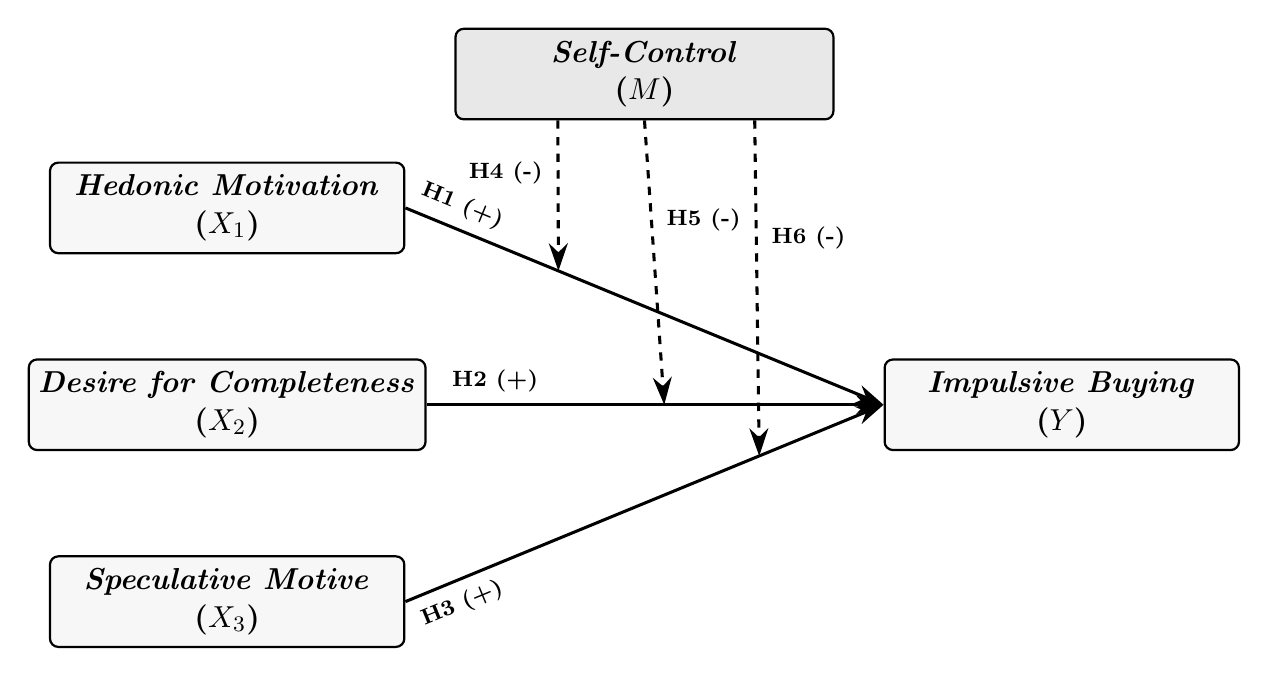
\begin{tikzpicture}[
  box/.style = {
    rectangle, draw=black, thick, fill=gray!6, rounded corners=3pt,
    minimum width=4.5cm, minimum height=1.15cm, align=center,
    font=\fontsize{11}{13.5}\selectfont\bfseries
  },
  modbox/.style = {
    rectangle, draw=black, thick, fill=gray!18, rounded corners=3pt,
    minimum width=4.8cm, minimum height=1.15cm, align=center,
    font=\fontsize{11}{13.5}\selectfont\bfseries
  },
  arrow/.style = {-{Stealth[length=3.5mm, width=2.4mm]}, line width=1.1pt},
  dasharrow/.style = {-{Stealth[length=3.5mm, width=2.4mm]}, line width=1.1pt, dashed}
]

  % Variabel Independen (X) di sebelah kiri (x = 0)
  \node[box] (x1) at (0, 2.5) {\emph{Hedonic Motivation}\\($X_1$)};
  \node[box] (x2) at (0, 0)   {\emph{Desire for Completeness}\\($X_2$)};
  \node[box] (x3) at (0, -2.5){\emph{Speculative Motive}\\($X_3$)};

  % Variabel Dependen (Y) di sebelah kanan (x = 10.6)
  \node[box] (y)  at (10.6, 0) {\emph{Impulsive Buying}\\($Y$)};

  % Variabel Moderasi (M) di atas tengah (x = 5.3, y = 4.2)
  \node[modbox] (m) at (5.3, 4.2) {\emph{Self-Control}\\($M$)};

  % Garis Pengaruh Langsung (H1, H2, H3)
  \draw[arrow] (x1.east) -- (y.west)
    node[pos=0.10, above=2pt, sloped, font=\footnotesize\bfseries, fill=white, inner sep=2pt] {H1 (+)};
  \draw[arrow] (x2.east) -- (y.west)
    node[pos=0.15, above=2pt, font=\footnotesize\bfseries, fill=white, inner sep=2pt] {H2 (+)};
  \draw[arrow] (x3.east) -- (y.west)
    node[pos=0.10, below=2pt, sloped, font=\footnotesize\bfseries, fill=white, inner sep=2pt] {H3 (+)};

  % Titik pertemuan moderasi yang terpisah secara horizontal (Parallel Tracks)
  \coordinate (mod1) at ($(x1.east)!0.32!(y.west)$);
  \coordinate (mod2) at ($(x2.east)!0.52!(y.west)$);
  \coordinate (mod3) at ($(x3.east)!0.74!(y.west)$);

  % Garis Pengaruh Moderasi (H4, H5, H6)
  \draw[dasharrow] ([xshift=-1.1cm]m.south) -- (mod1)
    node[pos=0.35, left=3pt, font=\footnotesize\bfseries, fill=white, inner sep=2pt] {H4 (-)};
  \draw[dasharrow] (m.south) -- (mod2)
    node[pos=0.35, right=3pt, font=\footnotesize\bfseries, fill=white, inner sep=2pt] {H5 (-)};
  \draw[dasharrow] ([xshift=1.4cm]m.south) -- (mod3)
    node[pos=0.35, right=3pt, font=\footnotesize\bfseries, fill=white, inner sep=2pt] {H6 (-)};

\end{tikzpicture}
}
\caption{Model Rerangka Konseptual Penelitian}
\label{fig:rerangka_penelitian}
\begin{flushleft}
  \footnotesize\textit{Keterangan:} Garis lurus menunjukkan pengaruh langsung (H1, H2, H3); Garis putus-putus menunjukkan efek moderasi kontrol diri yang memperlemah (H4, H5, H6).
\end{flushleft}
\end{figure}

% ============================================================
%  DAFTAR PUSTAKA
% ============================================================
\newpage
\renewcommand{\refname}{DAFTAR PUSTAKA}
\addcontentsline{toc}{section}{DAFTAR PUSTAKA}
\bibliography{references}

\end{document}
